\subsubsection{AES-256-GCM}
\small{The Advanced Encryption Standard is the symmetric encryption standard algorithm (NIST FIPS-197) almost worldwide since 2001, and it's known for high performances and security against cryptanalysis; in the application we employed its version with a 256 bits key, which has a security margin comparable to RSA with a 15360 bits key. Actually, since it's used in Galois/Counter Mode (GCM), it does not encrypt directly the plaintext, but it's instead used together with a 12 bytes initialization vector IV (which doesn't need to be secret, but unpredictable for every encryption, so the best choice is to pick it up randomly) to generate a pseudorandom keystream, which is then XORed to the plaintext: basically the block cipher simulates a stream cipher (so no padding is needed for the plaintext, whose length, thus, does not need to be a multiple of 16 bytes, like in direct encryption, which is a good thing, considering the 140 bytes limit for Android messages) which simulates a One Time Pad (OTP), the only cipher perfectly secure. Obviously AES-GCM is not perfectly secure because, frist, soon or later, a new key will be equal to one used in the past (not so soon though), second, the key is shorter than the plaintext and, third, the keystream is only pseudorandom. In addition to this the GCM mode generates also a 16 bytes Message Authentication Code (MAC) which is prepended to the ciphertext in order to provide an additional integrity check. Before the decryption (which needs of course the same IV and the same key) the message integrity is verified and, if it's not the case, an exception is raised and the command session is aborted. In GCM mode it's also possible to attach to the ciphertext some non-encrypted data (called Additional Authenticated Data, AAD) which are used along with the ciphertext itself to produce the MAC; in our case this feature is useless, so no AAD.\\The three pictures below show the encryption and the decryption under GMC (P = plaintext, K = key, C = ciphertext, A = AAD, T = MAC) and the AES encryption/decryption used to generate the keystream.}\\

\vspace{1cm}
\begin{center}
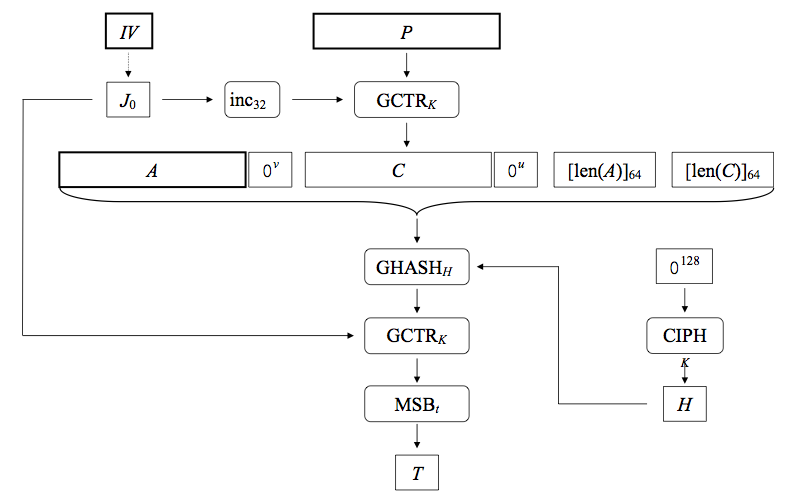
\includegraphics[scale=0.5]{images/aesgcmenc}\\

\vspace{1cm}
Picture 1: Encryption in GCM mode of operation\\
\clearpage
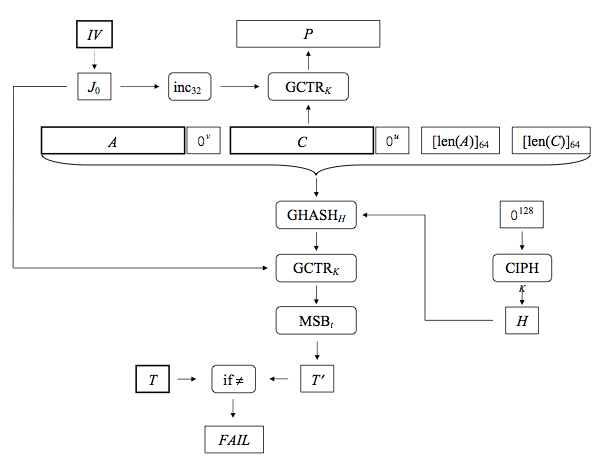
\includegraphics[scale=0.6]{images/aesgcmdec}\\

\vspace{0.5cm}
Picture 2: Decryption in GCM mode of operation\\

\vspace{2cm}
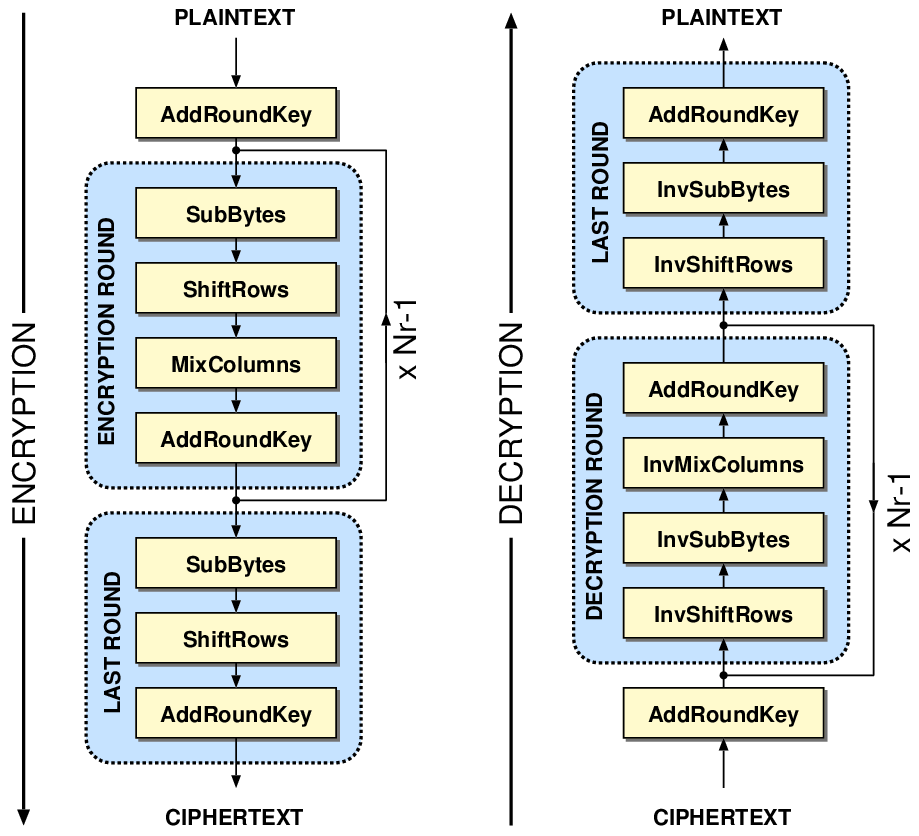
\includegraphics[scale=0.3]{images/aes}

\vspace{0.5cm}
Picture 3: Encryption/Decryption in AES\\
\end{center}